
%(BEGIN_QUESTION)
% Copyright 2006, Tony R. Kuphaldt, released under the Creative Commons Attribution License (v 1.0)
% This means you may do almost anything with this work of mine, so long as you give me proper credit

A solid metal cube measuring exactly 4 inches on a side is submerged in an open container filled with methanol.  The bottom of the cube is 10 inches down from the methanol's surface:

$$\includegraphics[width=15.5cm]{i00266x01.eps}$$

Based on your calculations of hydrostatic pressure (in PSI), determine the force applied to each side of the cube (in units of pounds), and the net, or {\it resultant} of these six forces (one force for each side of the cube).

Based on the figure for methanol density of 49.41 lb/ft$^{3}$, how much does 64 cubic inches of methanol (a 4" $\times$ 4" $\times$ 4" cube) happen to weigh?

\underbar{file i00266}
%(END_QUESTION)





%(BEGIN_ANSWER)

Force pushing up on cube's bottom face: 4.575 lb

Force pushing down on cube's top face: 2.745 lb

Average force pushing horizontally on each of the cube's four other faces: 3.660 lb

\vskip 10pt

Resultant force: 1.830 lb (upward) = weight of 64 in$^{3}$ of methanol @ 49.41 lb/ft$^{3}$.


%(END_ANSWER)





%(BEGIN_NOTES)


%INDEX% Physics, static fluids: buoyancy

%(END_NOTES)


